% !TeX root = ./main.tex
% !TEX program = xelatex

\documentclass[12pt]{article}
\usepackage{graphicx}
\usepackage{fullpage}
\usepackage{enumitem}
\usepackage{amsmath}
\usepackage{tikz}
\usetikzlibrary{arrows}
\usepackage{listings}
\usepackage{algorithm}
\usepackage[noend]{algpseudocode}
\usepackage{multicol}
\usepackage{microtype}
\usepackage{graphicx}
\usepackage[export]{adjustbox}
\usepackage{hyperref}
\hypersetup{
    colorlinks,
    citecolor=black,
    filecolor=black,
    linkcolor=black,
    urlcolor=black
}
\newcommand{\myparagraph}[1]{\paragraph{#1}\mbox{}\\}


%% Language and font encodings
\usepackage[utf8]{inputenc}
\usepackage{xunicode}
\usepackage{xltxtra}
\usepackage{amsfonts, amsmath}
\usepackage[english,greek]{babel}

%\usepackage{xgreek}

\setmainfont[Mapping=tex-text]{CMU Serif}
\begin{document}
\sloppy
\begin{titlepage}



\newcommand{\HRule}{\rule{\linewidth}{0.5mm}}
\center

\includegraphics[width=50mm,scale=0.5]{imgs/logo.png}\\[1cm]
\textsc{\LARGE ΕΘΝΙΚΟ ΜΕΤΣΟΒΙΟ ΠΟΛΥΤΕΧΝΕΙΟ}\\[0.05cm] % Name of your university/college
\textsc{\textbf{\Large ΣΧΟΛΗ ΗΛΕΚΤΡΟΛΟΓΩΝ ΜΗΧΑΝΙΚΩΝ \\ \& ΜΗΧΑΝΙΚΩΝ ΥΠΟΛΟΓΙΣΤΩΝ}}\\[1.cm] % Major heading such as course name

\vspace{05mm}
\HRule \\[0.4cm]
{ \huge \bfseries Άσκηση 2 - Προηγμένα Θέματα Αρχιτεκτονικής Υπολογιστών }\\[0.4cm] 
\HRule \\[1.5cm]
 
\center
{\Large Γρηγόριος Θανάσουλας \\ \vspace{1em} gregthanasoulas@gmail.com \\ \vspace{5mm} \Large A.M: 03114131} \\
\vspace{15mm}

{\large \today} % Date, change the \today to a set date if you want to be precise
\vfill

\end{titlepage}
\newpage
\tableofcontents
\newpage

\large{
\setcounter{tocdepth}{3}
\setcounter{secnumdepth}{3}
\section{Σκοπός}
\vspace{3mm}

Η άσκηση αυτή αποσκοπεί στη μελέτη της επίδοσης διαφορετικών branch predictors.
Για την αξιολόγηση τους γίνεται χρήση του εργαλείου PIN με τα παρακάτω
μετροπρογράμματα (SPEC CPU2006 benchmarks): 

\begin{enumerate}
  \item 403.gcc 
  \item 429.mcf 
  \item 434.zeusmp
  \item 436.cactusADM 
  \item 445.gobmk
  \item 450.soplex
  \item 456.hmmer
  \item 458.sjeng
  \item 459.GemsFDTD
  \item 471.omnetpp
  \item 473.astar
  \item 483.xalancbmk
\end{enumerate}}

\vspace{3mm}

\section{Πειραματική Αξιολόγηση}
\subsection{Μελέτη εντολών άλματος}
Στο παρόν τμήμα της εργασίας συλλέγουμε στατιστικά για το είδος εντολών άλματος των benchmarks που θα εκτελέσουμε.

\vspace{3mm}
   \begin{minipage}{\textwidth}
      \begin{center}
         \fbox{\textlatin{\textbf{\textit{403-gcc}}}}\\
         \vspace{3mm}
         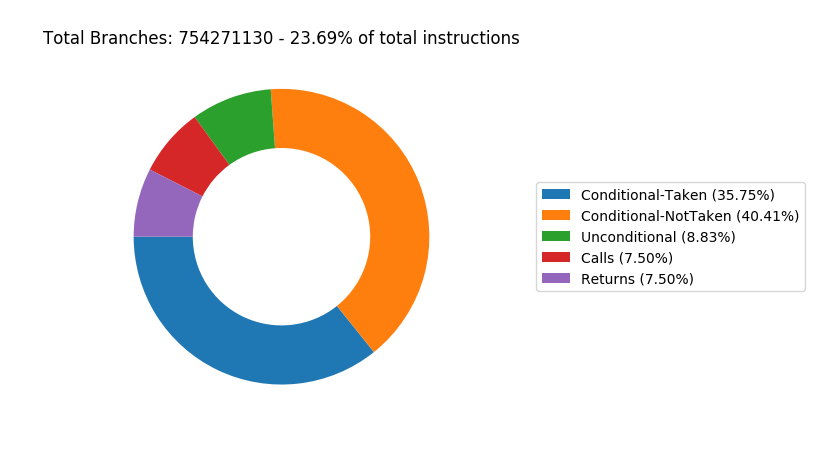
\includegraphics[width=0.9\textwidth, frame]{./graphs/4-1/403-gcc.png}
         \vspace{6mm}
      \end{center}
   \end{minipage}

   \begin{minipage}{\textwidth}
      \begin{center}
         \fbox{\textlatin{\textbf{\textit{429-mcf}}}}\\
         \vspace{3mm}
         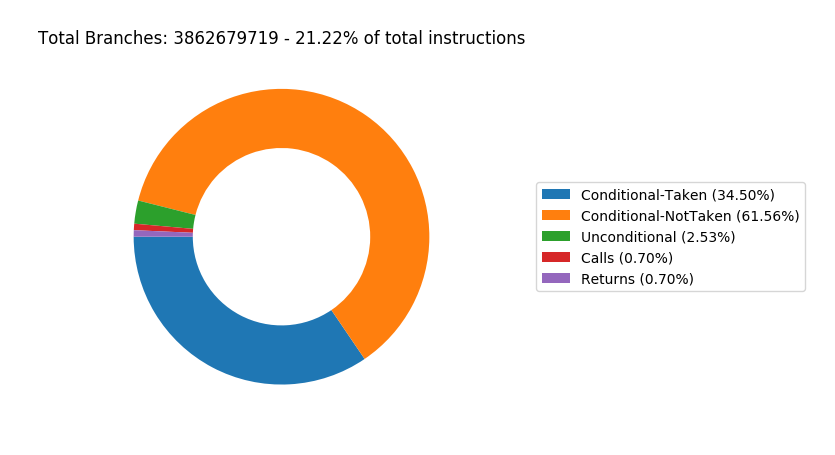
\includegraphics[width=0.9\textwidth, frame]{./graphs/4-1/429-mcf.png}
         \vspace{6mm}
      \end{center}
   \end{minipage}

   \begin{minipage}{\textwidth}
      \begin{center}
         \fbox{\textlatin{\textbf{\textit{434-zeusmp}}}}\\
         \vspace{3mm}
         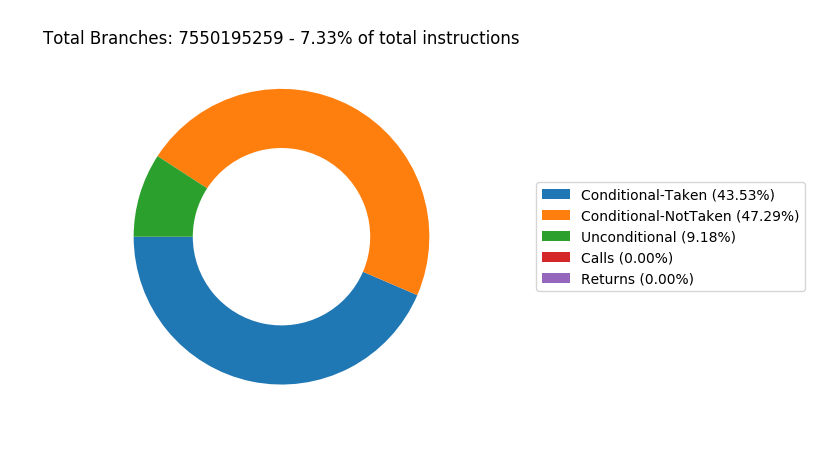
\includegraphics[width=0.9\textwidth, frame]{./graphs/4-1/434-zeusmp.png}
         \vspace{6mm}
      \end{center}
   \end{minipage}

   \begin{minipage}{\textwidth}
      \begin{center}
         \fbox{\textlatin{\textbf{\textit{436-cactusADM}}}}\\
         \vspace{3mm}
         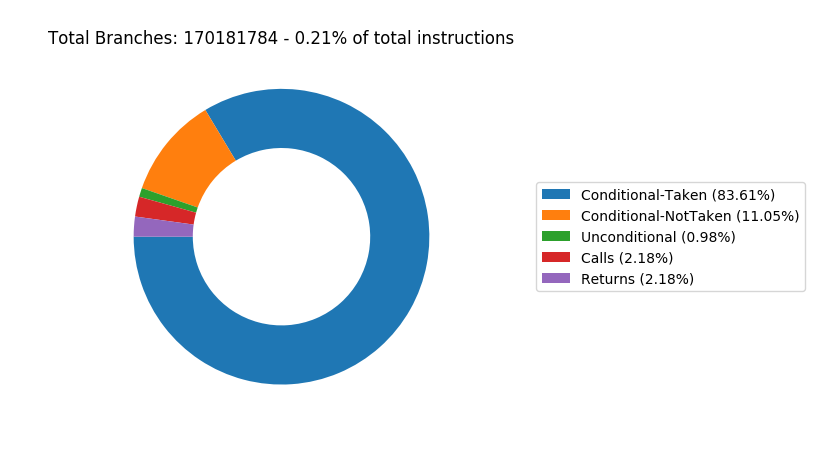
\includegraphics[width=0.9\textwidth, frame]{./graphs/4-1/436-cactusADM.png}
         \vspace{6mm}
      \end{center}
   \end{minipage}

   \begin{minipage}{\textwidth}
      \begin{center}
         \fbox{\textlatin{\textbf{\textit{445-gobmk}}}}\\
         \vspace{3mm}
         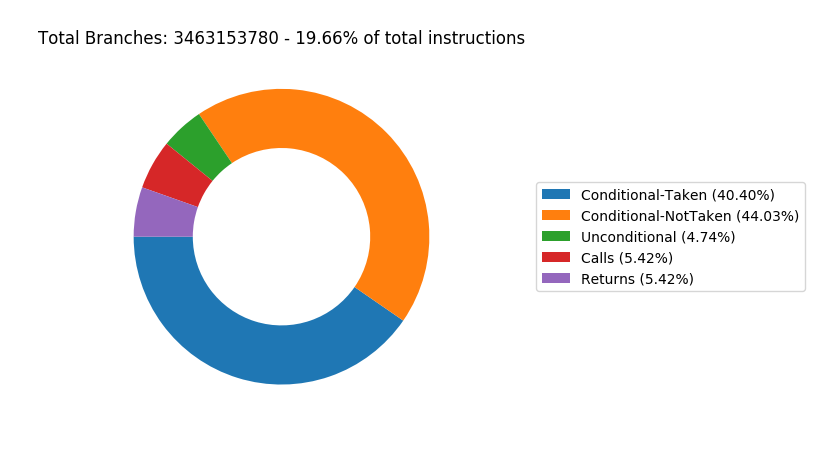
\includegraphics[width=0.9\textwidth, frame]{./graphs/4-1/445-gobmk.png}
         \vspace{6mm}
      \end{center}
   \end{minipage}

   \begin{minipage}{\textwidth}
      \begin{center}
         \fbox{\textlatin{\textbf{\textit{450-soplex}}}}\\
         \vspace{3mm}
         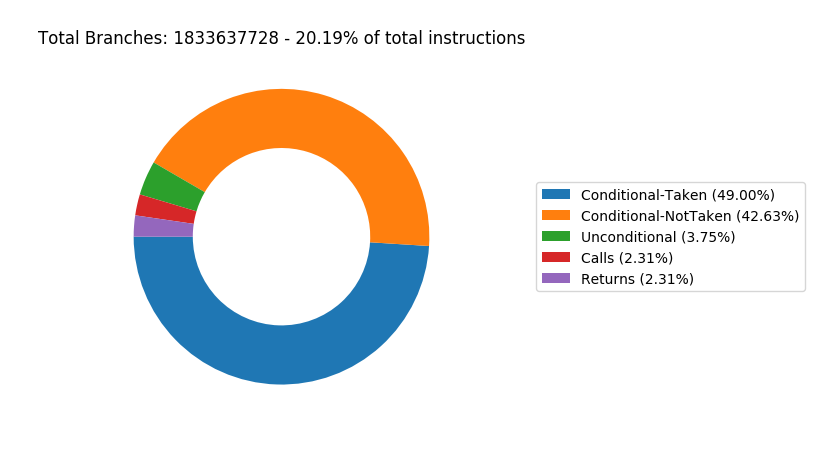
\includegraphics[width=0.9\textwidth, frame]{./graphs/4-1/450-soplex.png}
         \vspace{6mm}
      \end{center}
   \end{minipage}

   \begin{minipage}{\textwidth}
      \begin{center}
         \fbox{\textlatin{\textbf{\textit{456-hmmer}}}}\\
         \vspace{3mm}
         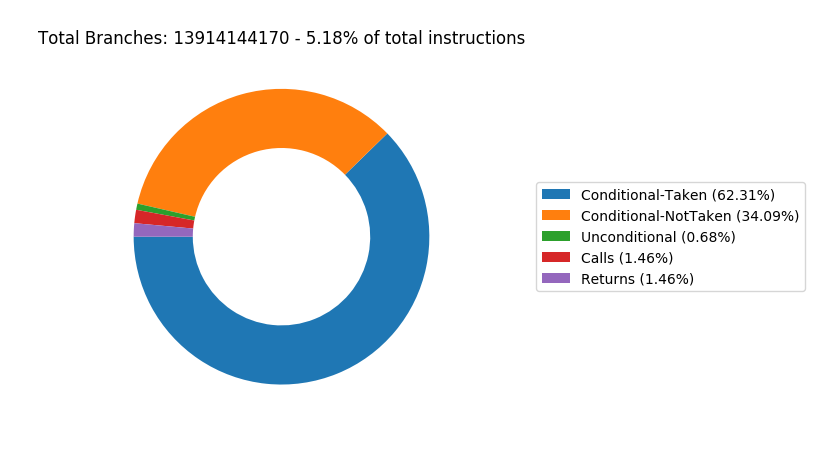
\includegraphics[width=0.9\textwidth, frame]{./graphs/4-1/456-hmmer.png}
         \vspace{6mm}
      \end{center}
   \end{minipage}

   \begin{minipage}{\textwidth}
      \begin{center}
         \fbox{\textlatin{\textbf{\textit{458-sjeng}}}}\\
         \vspace{3mm}
         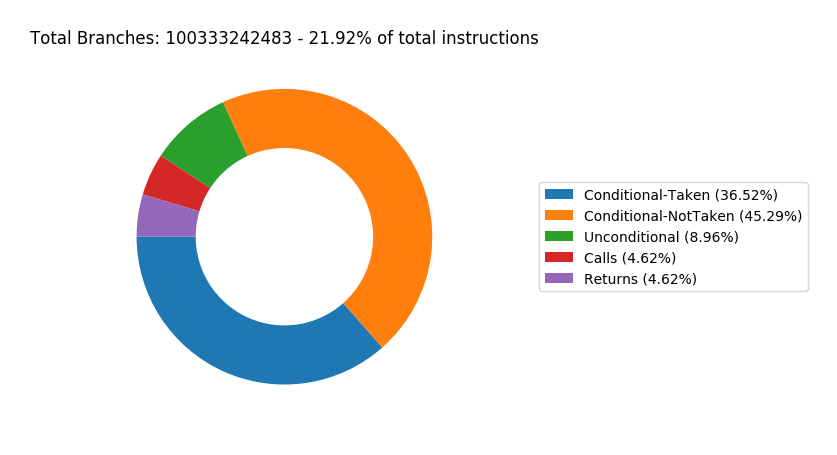
\includegraphics[width=0.9\textwidth, frame]{./graphs/4-1/458-sjeng.png}
         \vspace{6mm}
      \end{center}
   \end{minipage}

   \begin{minipage}{\textwidth}
      \begin{center}
         \fbox{\textlatin{\textbf{\textit{459-GemsFDTD}}}}\\
         \vspace{3mm}
         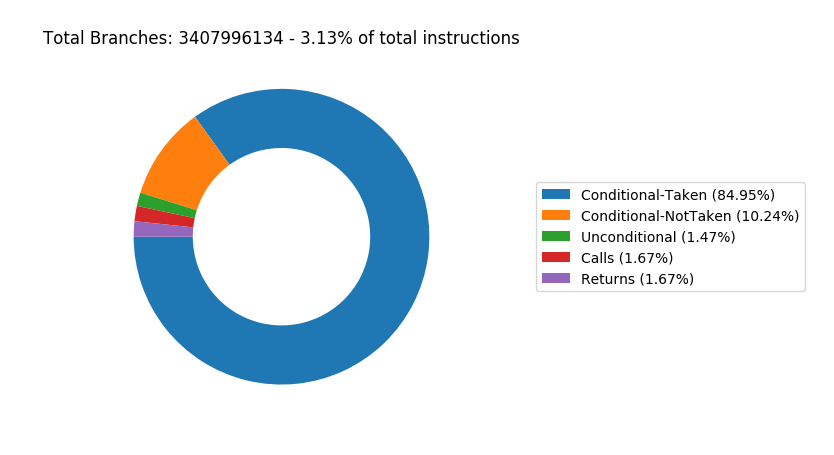
\includegraphics[width=0.9\textwidth, frame]{./graphs/4-1/459-GemsFDTD.png}
         \vspace{6mm}
      \end{center}
   \end{minipage}

   \begin{minipage}{\textwidth}
      \begin{center}
         \fbox{\textlatin{\textbf{\textit{471-omnetpp}}}}\\
         \vspace{3mm}
         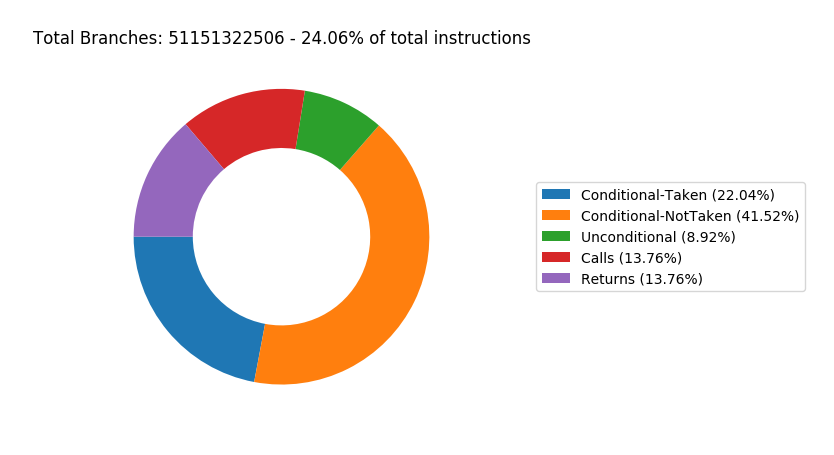
\includegraphics[width=0.9\textwidth, frame]{./graphs/4-1/471-omnetpp.png}
         \vspace{6mm}
      \end{center}
   \end{minipage}

   \begin{minipage}{\textwidth}
      \begin{center}
         \fbox{\textlatin{\textbf{\textit{473-astar}}}}\\
         \vspace{3mm}
         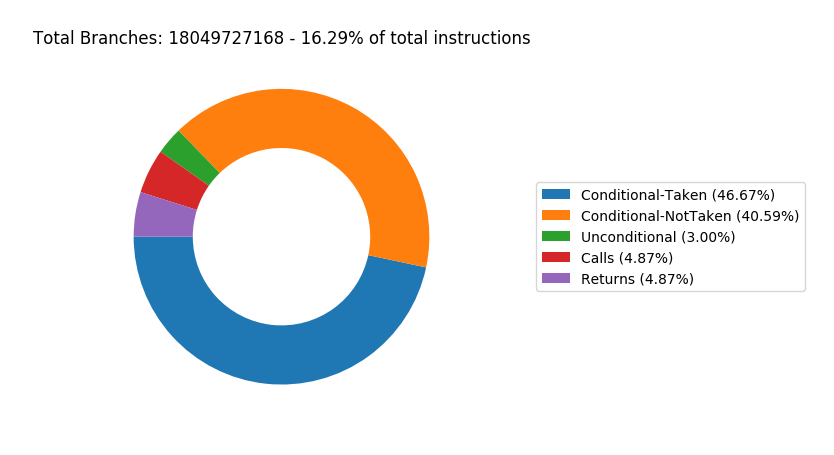
\includegraphics[width=0.9\textwidth, frame]{./graphs/4-1/473-astar.png}
         \vspace{6mm}
      \end{center}
   \end{minipage}

   \begin{minipage}{\textwidth}
      \begin{center}
         \fbox{\textlatin{\textbf{\textit{483-xalancbmk}}}}\\
         \vspace{3mm}
         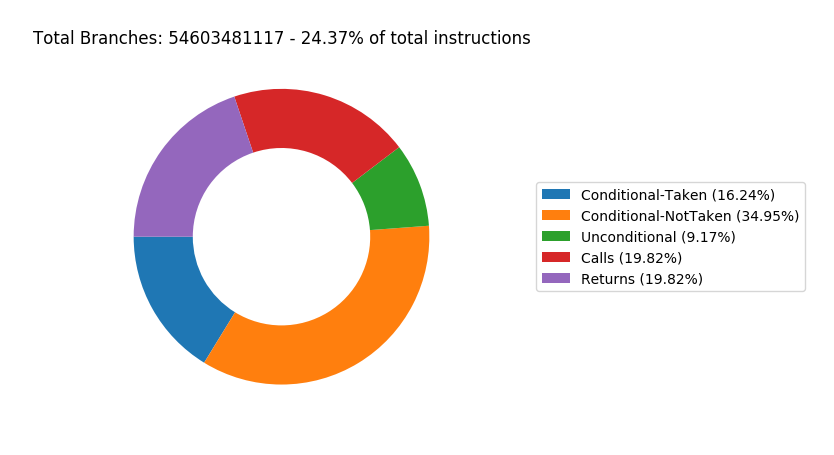
\includegraphics[width=0.9\textwidth, frame]{./graphs/4-1/483-xalancbmk.png}
         \vspace{6mm}
      \end{center}
   \end{minipage}

   \begin{minipage}{\textwidth}
      \begin{center}
         \vspace{3mm}
         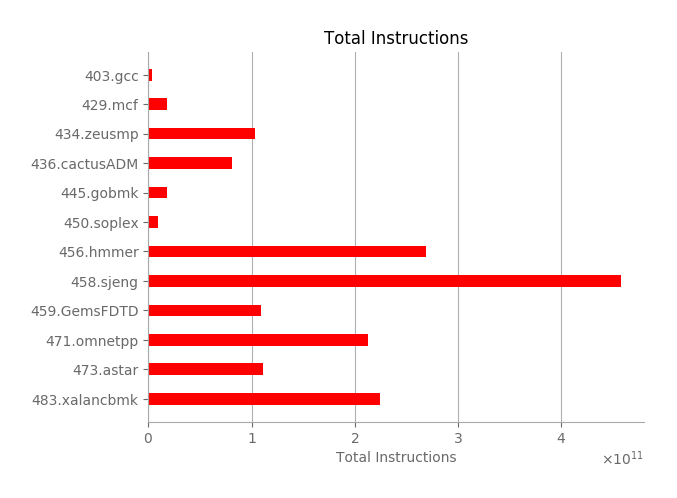
\includegraphics[width=0.8\textwidth, frame]{./graphs/4-1/total.png}
         \vspace{6mm}
      \end{center}
   \end{minipage}

   \paragraph{Συμπεράσματα - Σχόλια}

   Από τα παραπάνω διαγράμματα παρατηρούμε ότι στα μετροπρογράμματά μας οι
   εντολές άλματος αποτελούν ένα σημαντικό ποσοστό των συνολικών εντολών που
   εκτελούνται. Υπάρχουν benchmarks όπου οι εντολές άλματος είναι περίπου το
   20\%-30\% των συνολικών εντολών (403.gcc, 429.mcf, 445.gobmk, 450.soplex,
   458.sjeng, 483.xalancbmk, 473.astar) και άλλα όπου οι εντολές άλματος είναι
   σημαντικά λιγότερες κάτω του 5\% των συνολικών (459.GemsFDTD και
   436.cactusADM).
   
   Οσον αφορά την κατηγορία των αλμάτων, τα περισσότερα από αυτά τα είναι είτε
   Conditional Taken, είτε Conditional NotTaken. Αρκετά λιγότερα (συνολικά περί
   το 10\%) είναι τα Unconditional Branches, Calls, Returns.
   
   Τέλος, για το σύνολο των εντολών, όπως βλέπουμε στο σχετικό ραβδόγραμμα,
   υπάρχουν benchmarks με μικρό πλήθος εντολών (gcc, mcf, zeusmp, soplex, gobmk)
   και άλλα με αρκετά μεγάλο πλήθος εντολών τα οποία απαιτούν και μεγαλύτερο
   χρόνο εκτέλεσης (hmmer, sjeng, omnetop).
   
\newpage
\subsection{Μελέτη των N-bit Predictors}
\vspace{3mm}

\subsubsection{Μελέτη για σταθερό αριθμό BHT Entries}
Στο σημείο αυτό μελετάται η απόδοση των N-bit Predictors για διαφορετικές τιμές
του N = 1, 2, 3, 4, ενώ τα entries διατηρούνται σταθερά και ίσα με 16Κ.Τα N-bit
υλοποιούν ένα saturating up-down counter. Επιπλέον, υλοποιείται ένας predictor
με το κάτωθι FSM:

\begin{center}
   \vspace{3mm}
      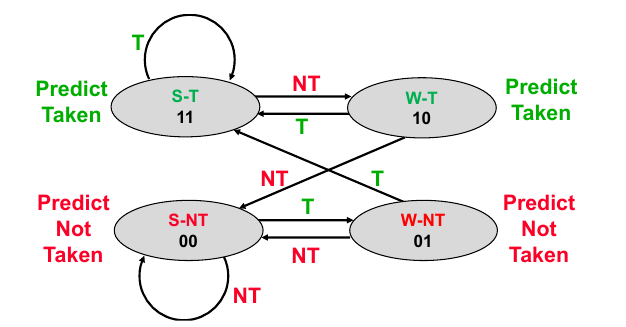
\includegraphics[width=0.65\textwidth, frame]{./imgs/fsm.png}
   \vspace{6mm}
\end{center}


\vspace{1em}    
Η σύγκριση των predictors γίνεται με βάση τα direction Mispredictions Per
Thousand Instructions (direction MPKI). Ακολουθούν τα διαγράμματα που
προέκυψαν και ο σχετικός σχολιασμός τους:

   \begin{minipage}{\textwidth}
      \begin{center}
         \fbox{\textlatin{\textbf{\textit{403-gcc}}}}\\
         \vspace{3mm}
         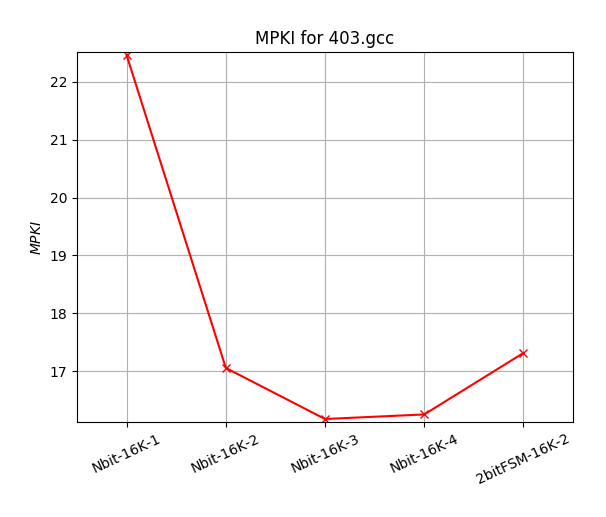
\includegraphics[width=0.65\textwidth, frame]{./graphs/4-2i/403-gcc.png}
         \vspace{6mm}
      \end{center}
   \end{minipage}

   \begin{minipage}{\textwidth}
      \begin{center}
         \fbox{\textlatin{\textbf{\textit{429-mcf}}}}\\
         \vspace{3mm}
         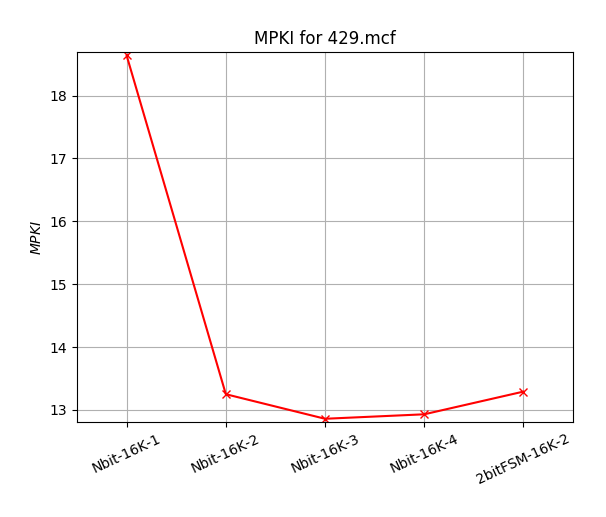
\includegraphics[width=0.65\textwidth, frame]{./graphs/4-2i/429-mcf.png}
         \vspace{6mm}
      \end{center}
   \end{minipage}

   \begin{minipage}{\textwidth}
      \begin{center}
         \fbox{\textlatin{\textbf{\textit{434-zeusmp}}}}\\
         \vspace{3mm}
         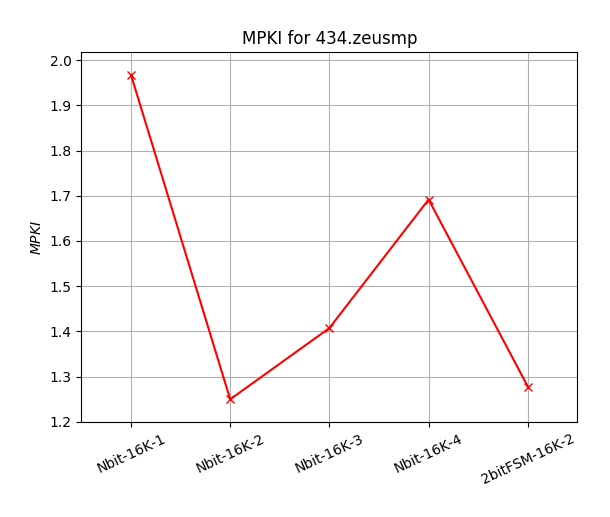
\includegraphics[width=0.65\textwidth, frame]{./graphs/4-2i/434-zeusmp.png}
         \vspace{6mm}
      \end{center}
   \end{minipage}

   \begin{minipage}{\textwidth}
      \begin{center}
         \fbox{\textlatin{\textbf{\textit{436-cactusADM}}}}\\
         \vspace{3mm}
         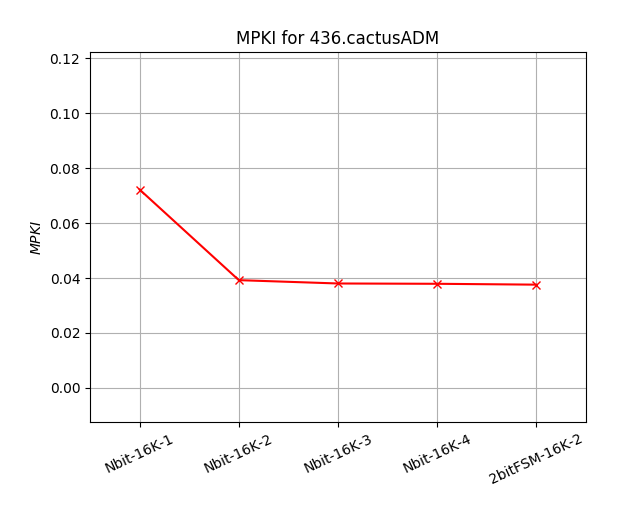
\includegraphics[width=0.65\textwidth, frame]{./graphs/4-2i/436-cactusADM.png}
         \vspace{6mm}
      \end{center}
   \end{minipage}

   \begin{minipage}{\textwidth}
      \begin{center}
         \fbox{\textlatin{\textbf{\textit{445-gobmk}}}}\\
         \vspace{3mm}
         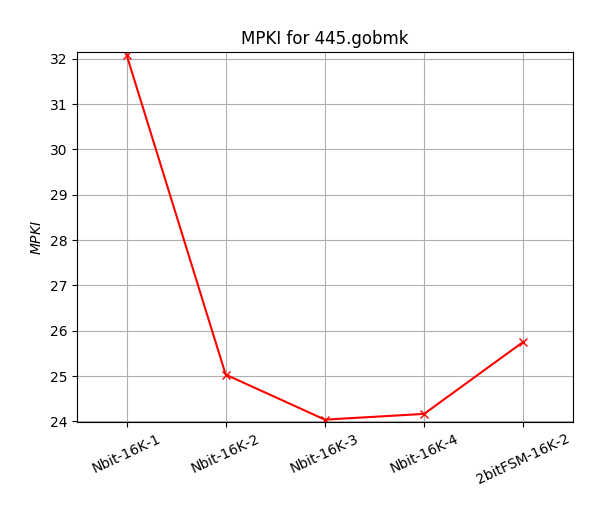
\includegraphics[width=0.65\textwidth, frame]{./graphs/4-2i/445-gobmk.png}
         \vspace{6mm}
      \end{center}
   \end{minipage}

   \begin{minipage}{\textwidth}
      \begin{center}
         \fbox{\textlatin{\textbf{\textit{450-soplex}}}}\\
         \vspace{3mm}
         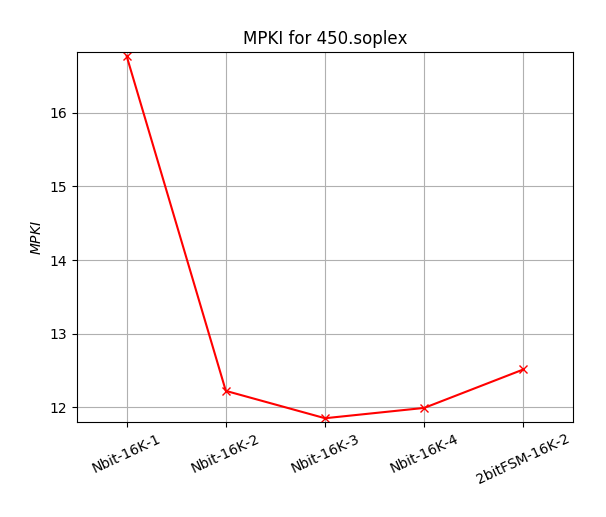
\includegraphics[width=0.65\textwidth, frame]{./graphs/4-2i/450-soplex.png}
         \vspace{6mm}
      \end{center}
   \end{minipage}

   \begin{minipage}{\textwidth}
      \begin{center}
         \fbox{\textlatin{\textbf{\textit{456-hmmer}}}}\\
         \vspace{3mm}
         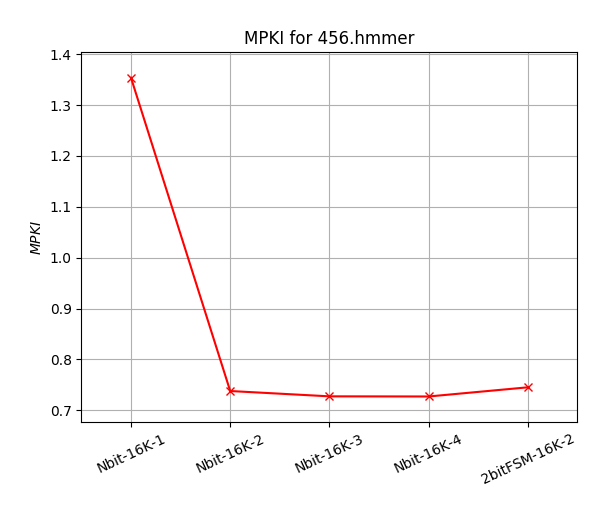
\includegraphics[width=0.65\textwidth, frame]{./graphs/4-2i/456-hmmer.png}
         \vspace{6mm}
      \end{center}
   \end{minipage}

   \begin{minipage}{\textwidth}
      \begin{center}
         \fbox{\textlatin{\textbf{\textit{458-sjeng}}}}\\
         \vspace{3mm}
         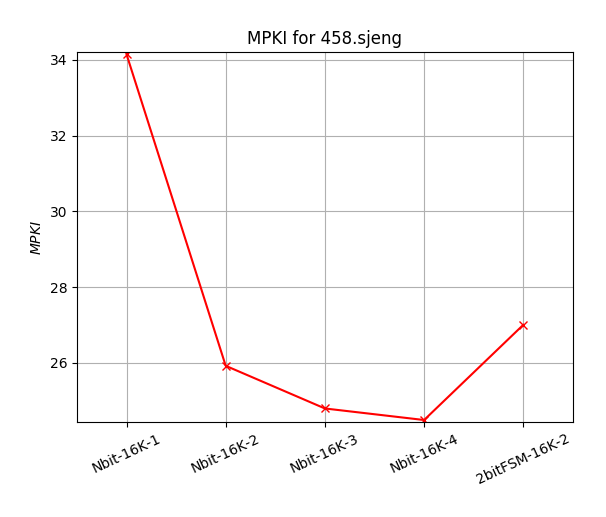
\includegraphics[width=0.65\textwidth, frame]{./graphs/4-2i/458-sjeng.png}
         \vspace{6mm}
      \end{center}
   \end{minipage}

   \begin{minipage}{\textwidth}
      \begin{center}
         \fbox{\textlatin{\textbf{\textit{459-GemsFDTD}}}}\\
         \vspace{3mm}
         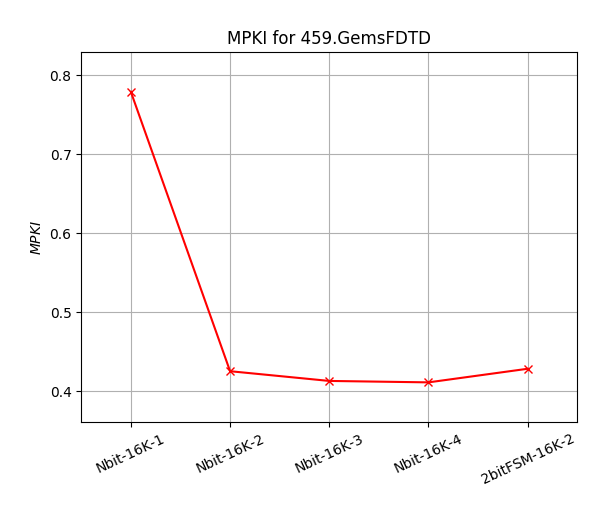
\includegraphics[width=0.65\textwidth, frame]{./graphs/4-2i/459-GemsFDTD.png}
         \vspace{6mm}
      \end{center}
   \end{minipage}

   \begin{minipage}{\textwidth}
      \begin{center}
         \fbox{\textlatin{\textbf{\textit{471-omnetpp}}}}\\
         \vspace{3mm}
         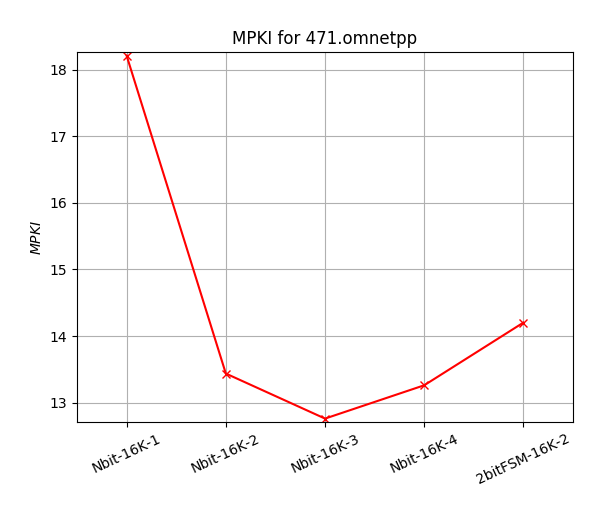
\includegraphics[width=0.65\textwidth, frame]{./graphs/4-2i/471-omnetpp.png}
         \vspace{6mm}
      \end{center}
   \end{minipage}

   \begin{minipage}{\textwidth}
      \begin{center}
         \fbox{\textlatin{\textbf{\textit{473-astar}}}}\\
         \vspace{3mm}
         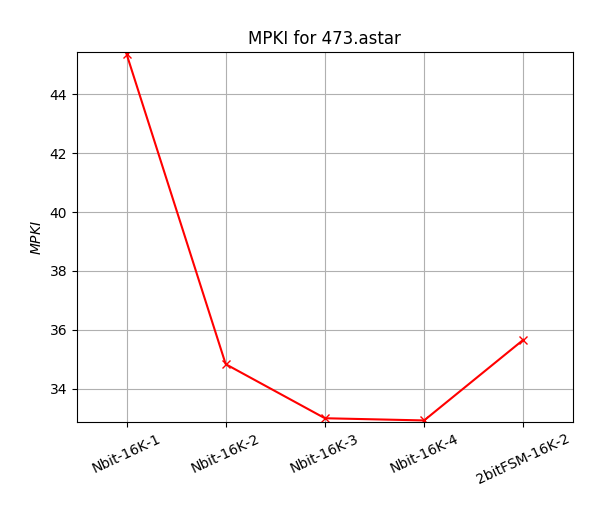
\includegraphics[width=0.65\textwidth, frame]{./graphs/4-2i/473-astar.png}
         \vspace{6mm}
      \end{center}
   \end{minipage}

   \begin{minipage}{\textwidth}
      \begin{center}
         \fbox{\textlatin{\textbf{\textit{483-xalancbmk}}}}\\
         \vspace{3mm}
         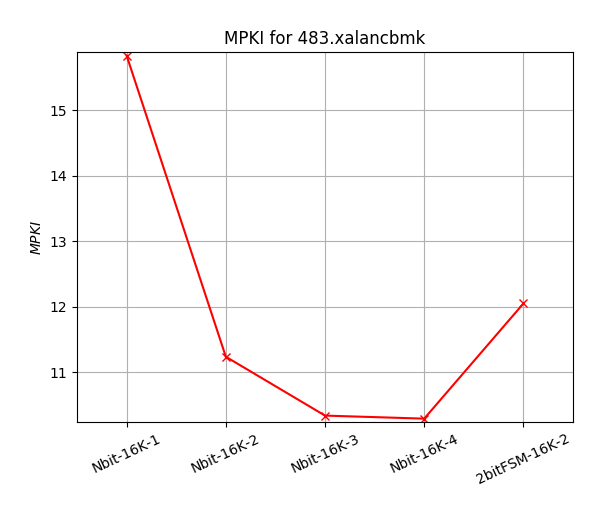
\includegraphics[width=0.65\textwidth, frame]{./graphs/4-2i/483-xalancbmk.png}
         \vspace{6mm}
      \end{center}
   \end{minipage}

   \begin{minipage}{\textwidth}
      \begin{center}
         \fbox{\textlatin{\textbf{\textit{Geometric Average}}}}\\
         \vspace{3mm}
         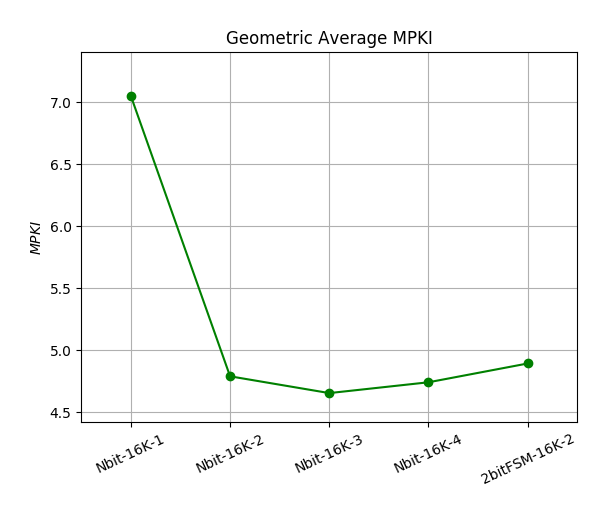
\includegraphics[width=0.65\textwidth, frame]{./graphs/4-2i/mean.png}
         \vspace{6mm}
      \end{center}
   \end{minipage}

\paragraph{Συμπεράσματα-Σχόλια}
    Από της μορφές των καμπυλών στα παραπάνω διαγράμματα παρατηρούμε πως 11 στα
    12 benchmarks παρουσιάζουν βελτίωση καθώς το πλήθος των bits του predictor
    αυξάνει, δηλάδή η μετρική dMPKI φθίνει καθώς τα bits αυξάνονται. Η μόνη
    διαφορετική ως προς την μορφή καμπύλη αντιστοιχεί στο μετρόπρόγραμμα
    434.zeusmp για το οποίο το μικρότερο MPKI αντιστοιχεί σε 2-bit predictor.
    Ωστόσο πρέπει να επισημάνουμε πως για το εν λόγω μετροπρόγραμμα η μεταβολή
    το MPKI είναι ήδη αρκετά χαμηλό και η μεταβολή του με τη χρήση διαφορετικών
    Nbit-Predictors είναι αρκετά μικρή (εύρος 1.2 εώς 2.0 Misses Per
    KILOInstructions), άρα δεν μας επηρεάζει και πολύ.

    Βοηθάει να αποκτήσουμε μία σαφώς πιο συνολική εικόνα και το διάγραμμα
    γεωμετρικών μέσων των παραπάνω τιμών, όπου εκεί επιβεβαιώνουμε τα
    προηγούμενα συμπεράσματα. Επιπλέον, να σημειώσουμε ότι το FSM που
    υλοποιήσαμε αποδίδει καλύτερα μονάχα σε σχέση με τον 1bit Predictor. Σαφώς η
    \textbf{καλύτερη επιλογή φαίνεται να είναι ο 4-bit Predictor}.


\newpage
\vspace{3mm}

\subsubsection{Μελέτη των N-bit Predictors για σταθερό πλήθος bits Hardware}
Στο σημείο αυτό επαναλαμβάνεται η μελέτη της απόδοσης των N-bit Predictors για
διαφορετικές τιμές του N = 1, 2, 2b, 4, με τη διαφοριά ότι θα ελέγξουμε την
επίδοση σε συνδυασμούς που αντιστοιχούν σε σταθερό hardware overhead 32Κ. \\

\noindent Ακολουθούν τα διαγράμματα που προέκυψαν και ο σχετικός σχολιασμός
τους:
\vspace{1em}

   \begin{minipage}{\textwidth}
      \begin{center}
         \fbox{\textlatin{\textbf{\textit{403-gcc}}}}\\
         \vspace{3mm}
         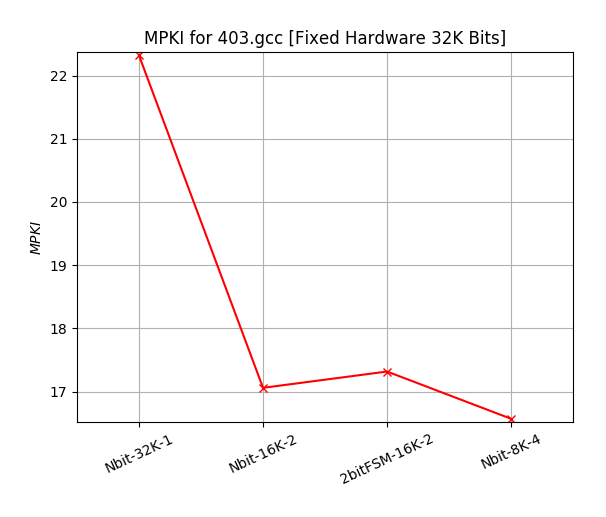
\includegraphics[width=0.65\textwidth, frame]{./graphs/4-2ii/403-gcc.png}
         \vspace{6mm}
      \end{center}
   \end{minipage}

   \begin{minipage}{\textwidth}
      \begin{center}
         \fbox{\textlatin{\textbf{\textit{429-mcf}}}}\\
         \vspace{3mm}
         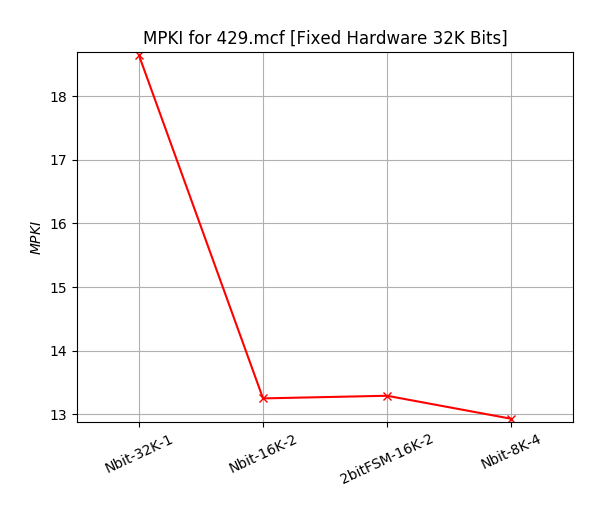
\includegraphics[width=0.65\textwidth, frame]{./graphs/4-2ii/429-mcf.png}
         \vspace{6mm}
      \end{center}
   \end{minipage}

   \begin{minipage}{\textwidth}
      \begin{center}
         \fbox{\textlatin{\textbf{\textit{434-zeusmp}}}}\\
         \vspace{3mm}
         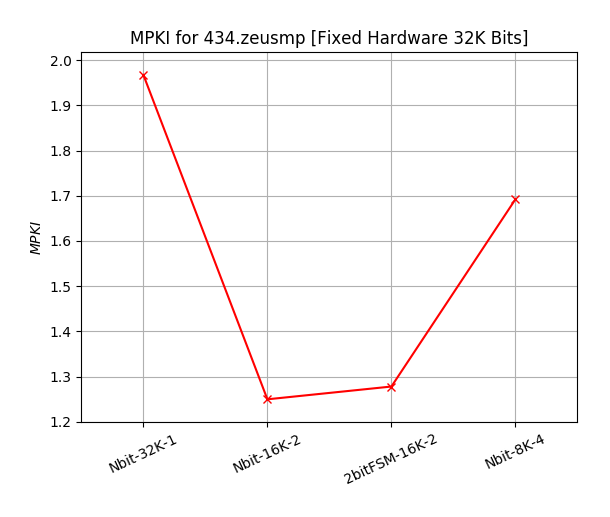
\includegraphics[width=0.65\textwidth, frame]{./graphs/4-2ii/434-zeusmp.png}
         \vspace{6mm}
      \end{center}
   \end{minipage}

   \begin{minipage}{\textwidth}
      \begin{center}
         \fbox{\textlatin{\textbf{\textit{436-cactusADM}}}}\\
         \vspace{3mm}
         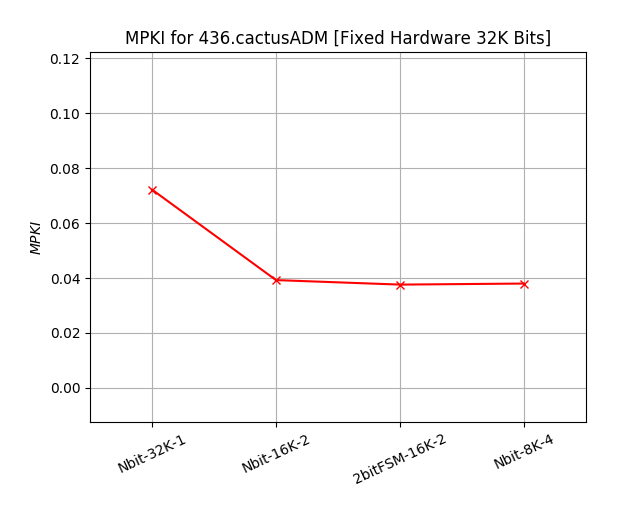
\includegraphics[width=0.65\textwidth, frame]{./graphs/4-2ii/436-cactusADM.png}
         \vspace{6mm}
      \end{center}
   \end{minipage}

   \begin{minipage}{\textwidth}
      \begin{center}
         \fbox{\textlatin{\textbf{\textit{445-gobmk}}}}\\
         \vspace{3mm}
         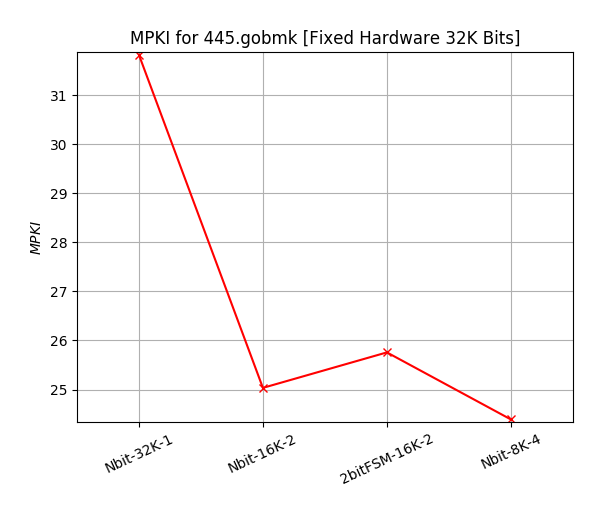
\includegraphics[width=0.65\textwidth, frame]{./graphs/4-2ii/445-gobmk.png}
         \vspace{6mm}
      \end{center}
   \end{minipage}

   \begin{minipage}{\textwidth}
      \begin{center}
         \fbox{\textlatin{\textbf{\textit{450-soplex}}}}\\
         \vspace{3mm}
         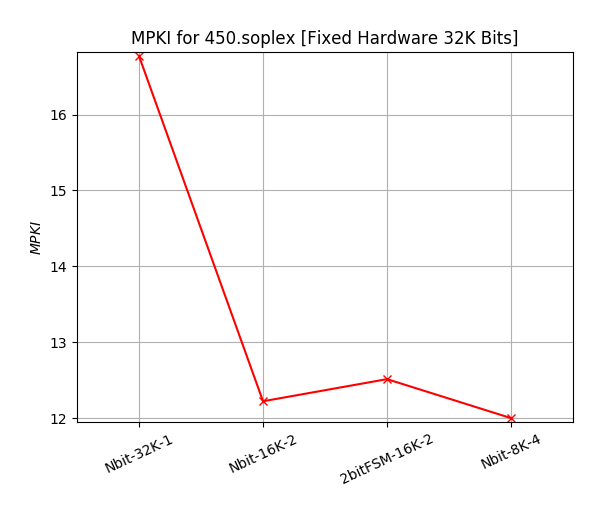
\includegraphics[width=0.65\textwidth, frame]{./graphs/4-2ii/450-soplex.png}
         \vspace{6mm}
      \end{center}
   \end{minipage}

   \begin{minipage}{\textwidth}
      \begin{center}
         \fbox{\textlatin{\textbf{\textit{456-hmmer}}}}\\
         \vspace{3mm}
         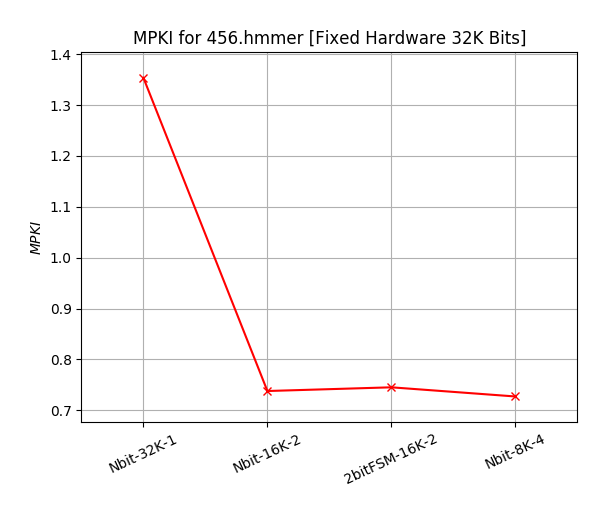
\includegraphics[width=0.65\textwidth, frame]{./graphs/4-2ii/456-hmmer.png}
         \vspace{6mm}
      \end{center}
   \end{minipage}

   \begin{minipage}{\textwidth}
      \begin{center}
         \fbox{\textlatin{\textbf{\textit{458-sjeng}}}}\\
         \vspace{3mm}
         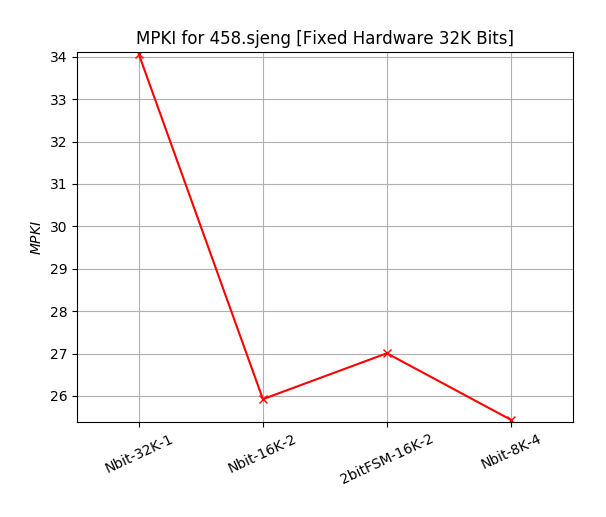
\includegraphics[width=0.65\textwidth, frame]{./graphs/4-2ii/458-sjeng.png}
         \vspace{6mm}
      \end{center}
   \end{minipage}

   \begin{minipage}{\textwidth}
      \begin{center}
         \fbox{\textlatin{\textbf{\textit{459-GemsFDTD}}}}\\
         \vspace{3mm}
         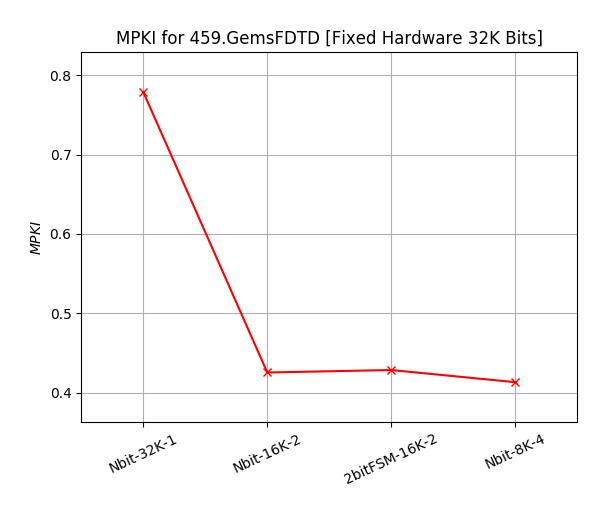
\includegraphics[width=0.65\textwidth, frame]{./graphs/4-2ii/459-GemsFDTD.png}
         \vspace{6mm}
      \end{center}
   \end{minipage}

   \begin{minipage}{\textwidth}
      \begin{center}
         \fbox{\textlatin{\textbf{\textit{471-omnetpp}}}}\\
         \vspace{3mm}
         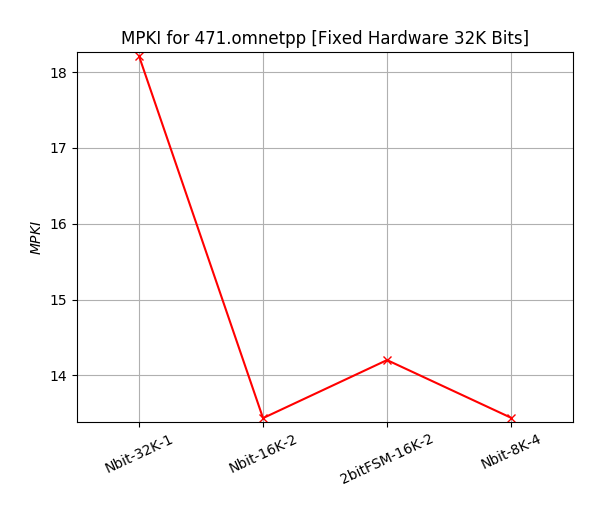
\includegraphics[width=0.65\textwidth, frame]{./graphs/4-2ii/471-omnetpp.png}
         \vspace{6mm}
      \end{center}
   \end{minipage}

   \begin{minipage}{\textwidth}
      \begin{center}
         \fbox{\textlatin{\textbf{\textit{473-astar}}}}\\
         \vspace{3mm}
         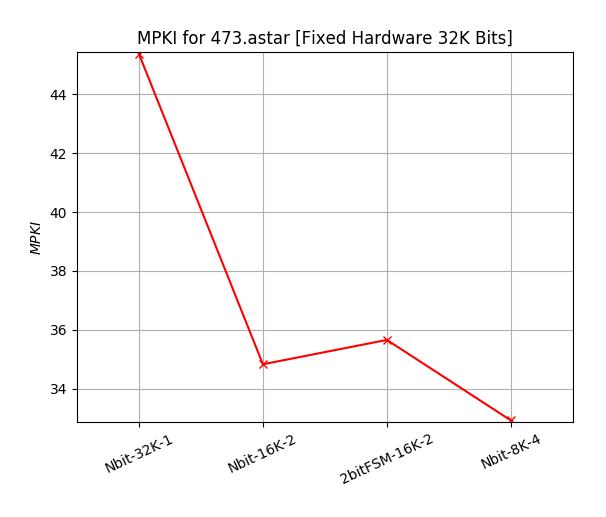
\includegraphics[width=0.65\textwidth, frame]{./graphs/4-2ii/473-astar.png}
         \vspace{6mm}
      \end{center}
   \end{minipage}

   \begin{minipage}{\textwidth}
      \begin{center}
         \fbox{\textlatin{\textbf{\textit{483-xalancbmk}}}}\\
         \vspace{3mm}
         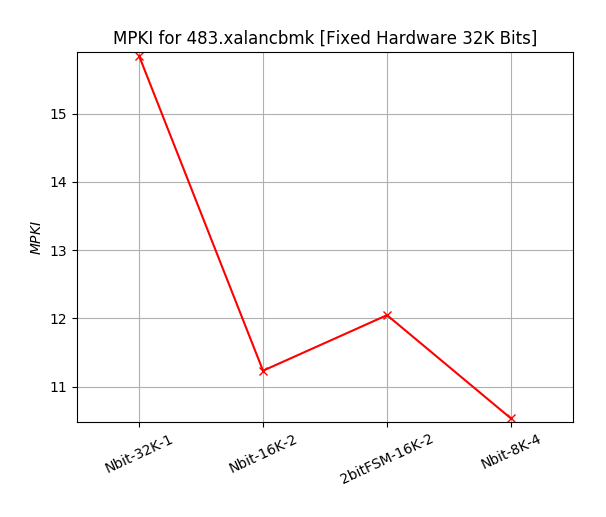
\includegraphics[width=0.65\textwidth, frame]{./graphs/4-2ii/483-xalancbmk.png}
         \vspace{6mm}
      \end{center}
   \end{minipage}

   \begin{minipage}{\textwidth}
      \begin{center}
         \fbox{\textlatin{\textbf{\textit{Geometric Average}}}}\\
         \vspace{3mm}
         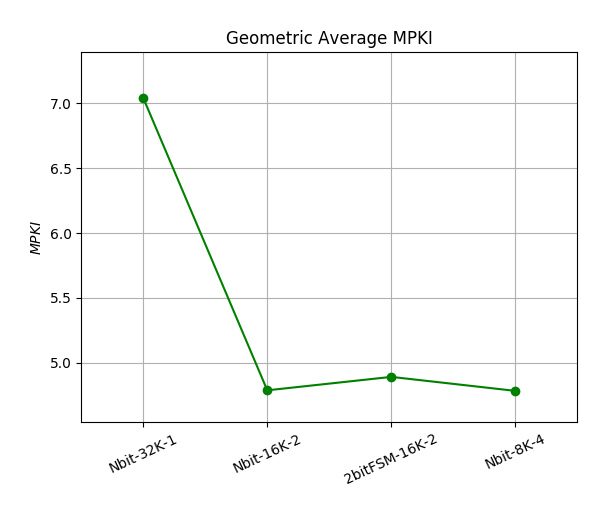
\includegraphics[width=0.65\textwidth, frame]{./graphs/4-2ii/mean.png}
         \vspace{6mm}
      \end{center}
   \end{minipage}

\paragraph{Συμπεράσματα-Σχόλια}
   Παρατηρούμε πως και στους νέους συνδυασμούς για σταθερό υλικό, η καμπύλες 
   μοιάζονυ με του προγηγούμενου ερωτήματος και τα συμπεράσματα είναι ανάλογα.

    Από της μορφές των καμπυλών στα παραπάνω διαγράμματα παρατηρούμε πως 11 στα
    12 benchmarks παρουσιάζουν βελτίωση καθώς το πλήθος των bits του predictor
    αυξάνει, δηλάδή η μετρική dMPKI φθίνει καθώς τα bits αυξάνονται, παρά την
    μείωση του πλήθος των predictors. Η μόνη διαφορετική ως προς την μορφή
    καμπύλη αντιστοιχεί στο μετρόπρόγραμμα 434.zeusmp για το οποίο το μικρότερο
    MPKI αντιστοιχεί σε 2-bit predictor.

   Από το διάγραμμα των γεωμετρικών μέσων μπορούμε να αποκτήσουμε μία συνολικότερη εποπτεία, 
   και να καταλήξουμε πως και σε αυτή την περίπτωση
    \textbf{καλύτερη επιλογή είναι ο 4-bit Predictor με 8Κ entries}.


\newpage
\subsection{Μελέτη του BTB}
\vspace{3mm}

Στο σημείο αυτό μελετάμε την απόδοση του BTB για διαφορες τιμές entries. 
Συγκεκριμένα έχουμε τους εξής συνδυασμούς:
\begin{itemize}
   \item 512 lines, associativity 1 
   \item 256 lines, associativity 2 
   \item 128 lines, associativity 4 
   \item 64 lines, associativity 8 
   \item 32 lines, associativity 4 
   \item 8 lines, associativity 8 
\end{itemize}

\vspace{1em}
Ακολουθούν τα διαγράμματα και ο σχετικός σχολιασμός:\vspace{1em}
\vspace{1em}    

   \begin{minipage}{\textwidth}
      \begin{center}
         \fbox{\textlatin{\textbf{\textit{403-gcc}}}}\\
         \vspace{3mm}
         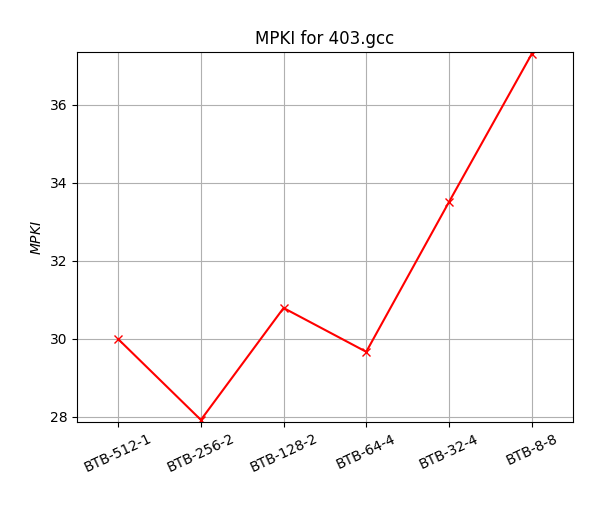
\includegraphics[width=0.65\textwidth, frame]{./graphs/4-3/403-gcc.png}
         \vspace{6mm}
      \end{center}
   \end{minipage}

   \begin{minipage}{\textwidth}
      \begin{center}
         \fbox{\textlatin{\textbf{\textit{429-mcf}}}}\\
         \vspace{3mm}
         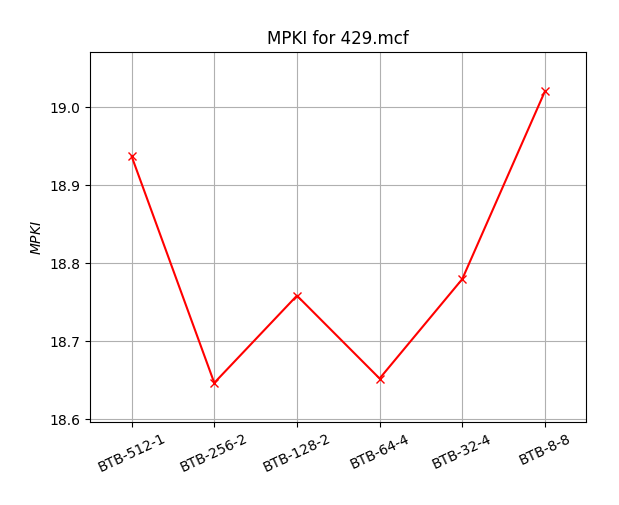
\includegraphics[width=0.65\textwidth, frame]{./graphs/4-3/429-mcf.png}
         \vspace{6mm}
      \end{center}
   \end{minipage}

   \begin{minipage}{\textwidth}
      \begin{center}
         \fbox{\textlatin{\textbf{\textit{434-zeusmp}}}}\\
         \vspace{3mm}
         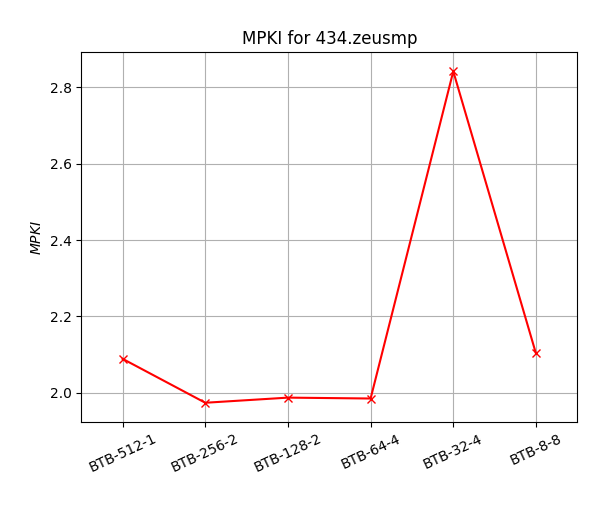
\includegraphics[width=0.65\textwidth, frame]{./graphs/4-3/434-zeusmp.png}
         \vspace{6mm}4
      \end{center}
   \end{minipage}

   \begin{minipage}{\textwidth}
      \begin{center}
         \fbox{\textlatin{\textbf{\textit{436-cactusADM}}}}\\
         \vspace{3mm}
         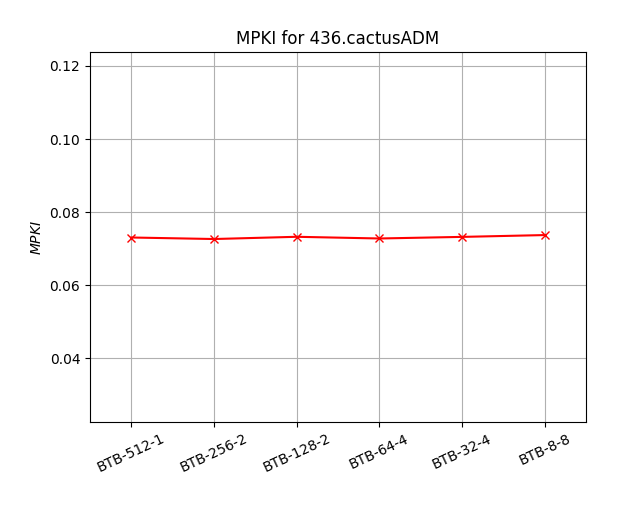
\includegraphics[width=0.65\textwidth, frame]{./graphs/4-3/436-cactusADM.png}
         \vspace{6mm}
      \end{center}
   \end{minipage}

   \begin{minipage}{\textwidth}
      \begin{center}
         \fbox{\textlatin{\textbf{\textit{445-gobmk}}}}\\
         \vspace{3mm}
         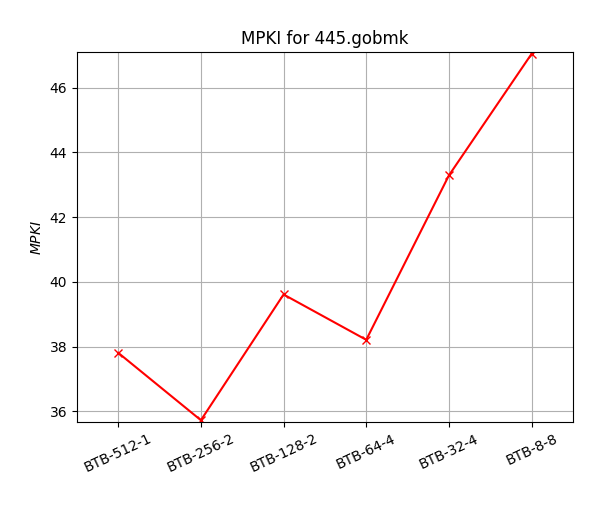
\includegraphics[width=0.65\textwidth, frame]{./graphs/4-3/445-gobmk.png}
         \vspace{6mm}
      \end{center}
   \end{minipage}

   \begin{minipage}{\textwidth}
      \begin{center}
         \fbox{\textlatin{\textbf{\textit{450-soplex}}}}\\
         \vspace{3mm}
         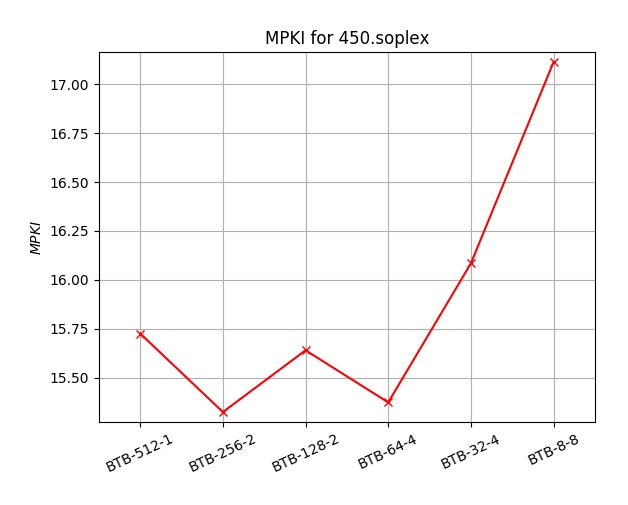
\includegraphics[width=0.65\textwidth, frame]{./graphs/4-3/450-soplex.png}
         \vspace{6mm}
      \end{center}
   \end{minipage}

   \begin{minipage}{\textwidth}
      \begin{center}
         \fbox{\textlatin{\textbf{\textit{456-hmmer}}}}\\
         \vspace{3mm}
         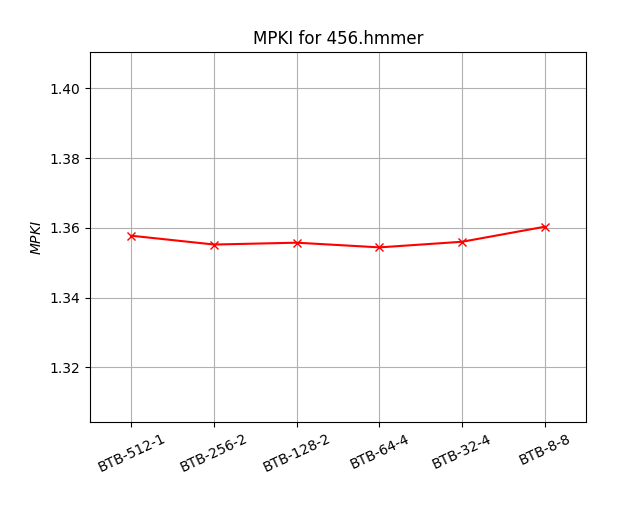
\includegraphics[width=0.65\textwidth, frame]{./graphs/4-3/456-hmmer.png}
         \vspace{6mm}
      \end{center}
   \end{minipage}

   \begin{minipage}{\textwidth}
      \begin{center}
         \fbox{\textlatin{\textbf{\textit{458-sjeng}}}}\\
         \vspace{3mm}
         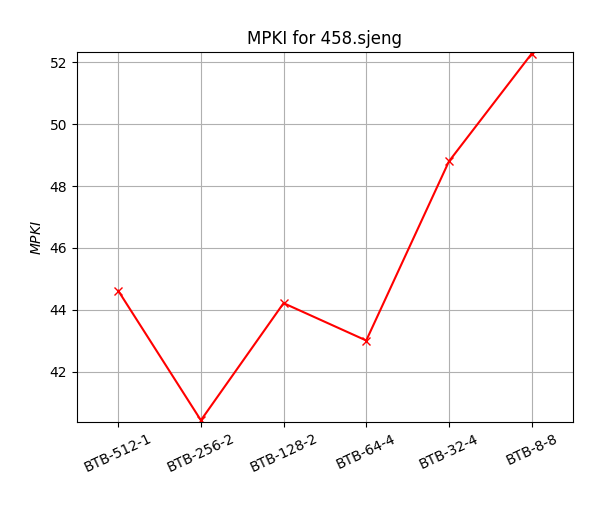
\includegraphics[width=0.65\textwidth, frame]{./graphs/4-3/458-sjeng.png}
         \vspace{6mm}
      \end{center}
   \end{minipage}

   \begin{minipage}{\textwidth}
      \begin{center}
         \fbox{\textlatin{\textbf{\textit{459-GemsFDTD}}}}\\
         \vspace{3mm}
         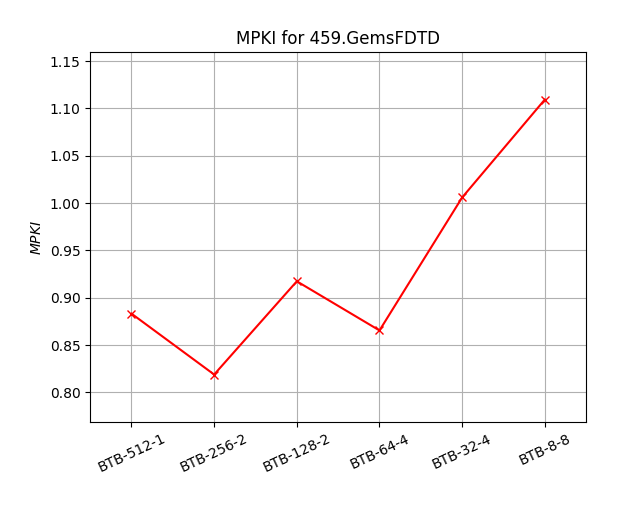
\includegraphics[width=0.65\textwidth, frame]{./graphs/4-3/459-GemsFDTD.png}
         \vspace{6mm}
      \end{center}
   \end{minipage}

   \begin{minipage}{\textwidth}
      \begin{center}
         \fbox{\textlatin{\textbf{\textit{471-omnetpp}}}}\\
         \vspace{3mm}
         \includegraphics[width=0.65\textwidth, frame]{./graphs/4-3/471-omnetpp.png}
         \vspace{6mm}
      \end{center}
   \end{minipage}

   \begin{minipage}{\textwidth}
      \begin{center}
         \fbox{\textlatin{\textbf{\textit{473-astar}}}}\\
         \vspace{3mm}
         \includegraphics[width=0.65\textwidth, frame]{./graphs/4-3/473-astar.png}
         \vspace{6mm}
      \end{center}
   \end{minipage}

   \begin{minipage}{\textwidth}
      \begin{center}
         \fbox{\textlatin{\textbf{\textit{483-xalancbmk}}}}\\
         \vspace{3mm}
         \includegraphics[width=0.65\textwidth, frame]{./graphs/4-3/483-xalancbmk.png}
         \vspace{6mm}
      \end{center}
   \end{minipage}

   \begin{minipage}{\textwidth}
      \begin{center}
         \fbox{\textlatin{\textbf{\textit{Geometric Average of MPKI}}}}\\
         \vspace{3mm}
         \includegraphics[width=0.65\textwidth, frame]{./graphs/4-3/mean.png}
         \vspace{6mm}
      \end{center}
   \end{minipage}


   \begin{minipage}{\textwidth}
      \begin{center}
         \fbox{\textlatin{\textbf{\textit{Benchmarks Overview}}}}\\
         \vspace{3mm}
         \includegraphics[width=\textwidth, frame]{./graphs/4-3/bar_chart.png}
         \vspace{6mm}
      \end{center}
   \end{minipage}

\paragraph{Συμπεράσματα-Σχόλια}
   Στα παραπάνω διαγράμματα χρησιμοποιούμε ως μετρική τα επιμέρους prediction misses +
   target misspredictions per KILOInstructions.

   Από τα επιμέρους διαγράμματα διαπιστώνουμε ότι για σταθερό πλήθος entries
   (table lines x associativity) η αύξηση του associativity επιφέρει βελτίωση.
   Την μιρκότερη τιμή misses επιτυγχάνουν οι συνδυασμοί BTB-256-2 και BTB-64-4.
   Μάλιστα ο BTB-256-2 φαίνεται να έχει καθολικό προβάδισμα στην απόδοση όπως
   βλέπουμε και στο διάγραμμα των γεωμετρικών μέσων. 

   Αξίζει να σημειώσουμε πως ο συνδυασμός BTB-8-8 έχει τη χειρότερη απόδοση, και
   άρα η υπερβολική αύξηση του associativity μειώνοντας τα table lines μετά από
   ένα όριο δε δρα βελτιωτικά.
  
   Τέλος από το ραβδόγραμμα Benchmarks Overview, όπου φαίνονται συγκεντρωτικά
   όλα τα παραπάνω και παρουσιάζονται τα total misspredictions per total
   instructions (\%), μπορούμε να επιβεβαιώσουμε ξανά ότι o BTB-256-2 έχει την
   καλύτερη επίδοση. Να σημειώσουμε σε αυτό το σημείο ότι στο διάγραμμα αυτό
   κάποια μετροπρογράμματα φαίνονται να έχουν υπερβολικά κάλή επίδοση (hmmer,
   cactusADM, etc), όμως αυτό οφείλεται εν μέρει και στο ότι γενικότερα έχουν
   μιρκό ποσοστό branches, όπως είδατε στο πρώτο τμήμα της παρούσας άσκησης.
   
   \textbf{Συνοπτικά, καλύτερη επιλογή είναι ο BTB Predictor με 512 entries, οργανωμένα σε 256 lines και associativity 2. }.


\newpage
\subsection{Μελέτη του RAS}
\vspace{3mm}

Στο σημείο αυτό μελετάμε την απόδοση του RAS για διαφορες τιμές entries.

\vspace{1em}    
Ακολουθούν τα διαγράμματα που προέκυψαν και ο σχετικός σχολιασμός
τους:

   \begin{minipage}{\textwidth}
      \begin{center}
         \fbox{\textlatin{\textbf{\textit{403-gcc}}}}\\
         \vspace{3mm}
         \includegraphics[width=0.65\textwidth, frame]{./graphs/4-4/403-gcc.png}
         \vspace{6mm}
      \end{center}
   \end{minipage}

   \begin{minipage}{\textwidth}
      \begin{center}
         \fbox{\textlatin{\textbf{\textit{429-mcf}}}}\\
         \vspace{3mm}
         \includegraphics[width=0.65\textwidth, frame]{./graphs/4-4/429-mcf.png}
         \vspace{6mm}
      \end{center}
   \end{minipage}

   \begin{minipage}{\textwidth}
      \begin{center}
         \fbox{\textlatin{\textbf{\textit{434-zeusmp}}}}\\
         \vspace{3mm}
         \includegraphics[width=0.65\textwidth, frame]{./graphs/4-4/434-zeusmp.png}
         \vspace{6mm}4
      \end{center}
   \end{minipage}

   \begin{minipage}{\textwidth}
      \begin{center}
         \fbox{\textlatin{\textbf{\textit{436-cactusADM}}}}\\
         \vspace{3mm}
         \includegraphics[width=0.65\textwidth, frame]{./graphs/4-4/436-cactusADM.png}
         \vspace{6mm}
      \end{center}
   \end{minipage}

   \begin{minipage}{\textwidth}
      \begin{center}
         \fbox{\textlatin{\textbf{\textit{445-gobmk}}}}\\
         \vspace{3mm}
         \includegraphics[width=0.65\textwidth, frame]{./graphs/4-4/445-gobmk.png}
         \vspace{6mm}
      \end{center}
   \end{minipage}

   \begin{minipage}{\textwidth}
      \begin{center}
         \fbox{\textlatin{\textbf{\textit{450-soplex}}}}\\
         \vspace{3mm}
         \includegraphics[width=0.65\textwidth, frame]{./graphs/4-4/450-soplex.png}
         \vspace{6mm}
      \end{center}
   \end{minipage}

   \begin{minipage}{\textwidth}
      \begin{center}
         \fbox{\textlatin{\textbf{\textit{456-hmmer}}}}\\
         \vspace{3mm}
         \includegraphics[width=0.65\textwidth, frame]{./graphs/4-4/456-hmmer.png}
         \vspace{6mm}
      \end{center}
   \end{minipage}

   \begin{minipage}{\textwidth}
      \begin{center}
         \fbox{\textlatin{\textbf{\textit{458-sjeng}}}}\\
         \vspace{3mm}
         \includegraphics[width=0.65\textwidth, frame]{./graphs/4-4/458-sjeng.png}
         \vspace{6mm}
      \end{center}
   \end{minipage}

   \begin{minipage}{\textwidth}
      \begin{center}
         \fbox{\textlatin{\textbf{\textit{459-GemsFDTD}}}}\\
         \vspace{3mm}
         \includegraphics[width=0.65\textwidth, frame]{./graphs/4-4/459-GemsFDTD.png}
         \vspace{6mm}
      \end{center}
   \end{minipage}

   \begin{minipage}{\textwidth}
      \begin{center}
         \fbox{\textlatin{\textbf{\textit{471-omnetpp}}}}\\
         \vspace{3mm}
         \includegraphics[width=0.65\textwidth, frame]{./graphs/4-4/471-omnetpp.png}
         \vspace{6mm}
      \end{center}
   \end{minipage}

   \begin{minipage}{\textwidth}
      \begin{center}
         \fbox{\textlatin{\textbf{\textit{473-astar}}}}\\
         \vspace{3mm}
         \includegraphics[width=0.65\textwidth, frame]{./graphs/4-4/473-astar.png}
         \vspace{6mm}
      \end{center}
   \end{minipage}

   \begin{minipage}{\textwidth}
      \begin{center}
         \fbox{\textlatin{\textbf{\textit{483-xalancbmk}}}}\\
         \vspace{3mm}
         \includegraphics[width=0.65\textwidth, frame]{./graphs/4-4/483-xalancbmk.png}
         \vspace{6mm}
      \end{center}
   \end{minipage}


   \begin{minipage}{\textwidth}
      \begin{center}
         \fbox{\textlatin{\textbf{\textit{Geometric Average of MPKI}}}}\\
         \vspace{3mm}
         \includegraphics[width=0.65\textwidth, frame]{./graphs/4-4/mean.png}
         \vspace{6mm}
      \end{center}
   \end{minipage}

\paragraph{Συμπεράσματα-Σχόλια}
   

   Για αριθμό εγγραφών στη RAS ίσο με 1, παρατηρούμε σε σχεδόν όλα τα benchmarks
   πολύ υψηλό MPKI. Μόλις το RAS κάνει χρήση 2 εγγραφών, είναι εμφανής η
   σημαντική μείωση του MPKI. Για μεταβολή από 2 σε 4 εγγραφές, παρατηρούμε και
   πάλι σχεδόν σε όλα τα μετροπρογράμματα μείωση του MPKI, όπως είναι επιθυμητό.
   Για παραπάνω entries, τα MPKI μειώνονται μεν αλλά πλέον σχετικά λίγο, είτε
   παραμένουν σταθερά. Σε κάθε περίπτωση με την αύξηση των εγγραφών οδηγούμαστε
   σε βελτίωση της επίδοσης, ωστόσο από ένα σημείο και πέρα η περεταίρω αύξηση
   δεν έχει νόημα καθώς η επίδοση δεν βελτιώνονται δραστικά αναλογικά με την
   αύξηση του υλικού που πραγματοποιούμε. 

   Με βάση τα παραπάνω, οι επιλογή 16 ή 32 ή 64 εγγραφών είναι αρκετά καλή
   επιλογή. Αν λαμβάναμε υπ’ όψιν και το κόστος του σχετικού υλικού, τότε
   ενδεχομένως να έπρεπε να περιοριστούμε στο ελάχιστο υλικό και άρα να
   επιλέξουμε 16 εγγραφές RAS.
   
   \textbf{Συνοπτικά, καλύτερη επιλογή είναι 16 εγγραφές στην RAS}.
\newpage
\subsection{Μελέτη διαφορετικών Branch Predictors}
\vspace{3mm}

Στο σημείο αυτό μελετάμε την απόδοση διαφορετικών predicotrs στο σύνολο των
μετροπρογραμμάτων. Οι Predictors που συγκρίνονται είναι οι παρακάτω:

\begin{flushleft}
\begin{enumerate}
   \item Static Taken Predictor
   \item BTFNTPredictor
   \item Pentium-M
   \item Nbit-8K-4bit 
   \item LocalHistory-PHT(8K,2bit)-BHT(2K,8bit)
   \item LocalHistory-PHT(8K,2bit)-BHT(4K,4bit)
   \item GlobalHistory-PHT(16K,2bit)-BHR(5bit)
   \item GlobalHistory-PHT(8K,4bit)-BHR(5bit)
   \item GlobalHistory-PHT(8K,4bit)-BHR(10bit)
   \item GlobalHistory-PHT(16K,2bit)-BHR(10bit)
   \item Tournament(Nbit-8K-2bit, Nbit-4K-4bit)
   \item Tournament(GlobalHistory-PHT(4K,4bit)-BHR(2bit), Nbit-8K-2bit)
   \item Tournament(GlobalHistory-PHT(8K,2bit)-BHR(2bit), LocalHistory-PHT(2K,4bit)-BHT(4K,2bit))
   \item Tournament(Nbit-8K-2bit, GlobalHistory-PHT(8K,2bit)-BHR(5bit))
   \item Tournament(Nbit-2K-8bit, LocalHistory-PHT(2K,4bit)-BHT(4K,2bit))
   \item ALPHA-PREDICTOR
\end{enumerate}
\end{flushleft}

\vspace{1em}    
Ακολουθούν τα διαγράμματα που προέκυψαν και ο σχετικός σχολιασμός
τους:
\vspace{1em}    

   \begin{minipage}{\textwidth}
      \begin{center}
         \fbox{\textlatin{\textbf{\textit{403-gcc}}}}\\
         \vspace{3mm}
         \includegraphics[width=0.9\textwidth, frame]{./graphs/4-5/403-gcc.png}
         \vspace{6mm}
      \end{center}
   \end{minipage}

   \begin{minipage}{\textwidth}
      \begin{center}
         \fbox{\textlatin{\textbf{\textit{429-mcf}}}}\\
         \vspace{3mm}
         \includegraphics[width=0.9\textwidth, frame]{./graphs/4-5/429-mcf.png}
         \vspace{6mm}
      \end{center}
   \end{minipage}

   \begin{minipage}{\textwidth}
      \begin{center}
         \fbox{\textlatin{\textbf{\textit{434-zeusmp}}}}\\
         \vspace{3mm}
         \includegraphics[width=0.9\textwidth, frame]{./graphs/4-5/434-zeusmp.png}
         \vspace{6mm}4
      \end{center}
   \end{minipage}

   \begin{minipage}{\textwidth}
      \begin{center}
         \fbox{\textlatin{\textbf{\textit{436-cactusADM}}}}\\
         \vspace{3mm}
         \includegraphics[width=0.9\textwidth, frame]{./graphs/4-5/436-cactusADM.png}
         \vspace{6mm}
      \end{center}
   \end{minipage}

   \begin{minipage}{\textwidth}
      \begin{center}
         \fbox{\textlatin{\textbf{\textit{445-gobmk}}}}\\
         \vspace{3mm}
         \includegraphics[width=0.9\textwidth, frame]{./graphs/4-5/445-gobmk.png}
         \vspace{6mm}
      \end{center}
   \end{minipage}

   \begin{minipage}{\textwidth}
      \begin{center}
         \fbox{\textlatin{\textbf{\textit{450-soplex}}}}\\
         \vspace{3mm}
         \includegraphics[width=0.9\textwidth, frame]{./graphs/4-5/450-soplex.png}
         \vspace{6mm}
      \end{center}
   \end{minipage}

   \begin{minipage}{\textwidth}
      \begin{center}
         \fbox{\textlatin{\textbf{\textit{456-hmmer}}}}\\
         \vspace{3mm}
         \includegraphics[width=0.9\textwidth, frame]{./graphs/4-5/456-hmmer.png}
         \vspace{6mm}
      \end{center}
   \end{minipage}

   \begin{minipage}{\textwidth}
      \begin{center}
         \fbox{\textlatin{\textbf{\textit{458-sjeng}}}}\\
         \vspace{3mm}
         \includegraphics[width=0.9\textwidth, frame]{./graphs/4-5/458-sjeng.png}
         \vspace{6mm}
      \end{center}
   \end{minipage}

   \begin{minipage}{\textwidth}
      \begin{center}
         \fbox{\textlatin{\textbf{\textit{459-GemsFDTD}}}}\\
         \vspace{3mm}
         \includegraphics[width=0.9\textwidth, frame]{./graphs/4-5/459-GemsFDTD.png}
         \vspace{6mm}
      \end{center}
   \end{minipage}

   \begin{minipage}{\textwidth}
      \begin{center}
         \fbox{\textlatin{\textbf{\textit{471-omnetpp}}}}\\
         \vspace{3mm}
         \includegraphics[width=0.9\textwidth, frame]{./graphs/4-5/471-omnetpp.png}
         \vspace{6mm}
      \end{center}
   \end{minipage}

   \begin{minipage}{\textwidth}
      \begin{center}
         \fbox{\textlatin{\textbf{\textit{473-astar}}}}\\
         \vspace{3mm}
         \includegraphics[width=0.9\textwidth, frame]{./graphs/4-5/473-astar.png}
         \vspace{6mm}
      \end{center}
   \end{minipage}

   \begin{minipage}{\textwidth}
      \begin{center}
         \fbox{\textlatin{\textbf{\textit{483-xalancbmk}}}}\\
         \vspace{3mm}
         \includegraphics[width=0.9\textwidth, frame]{./graphs/4-5/483-xalancbmk.png}
         \vspace{6mm}
      \end{center}
   \end{minipage}


   \begin{minipage}{\textwidth}
      \begin{center}
         \fbox{\textlatin{\textbf{\textit{Geometric Average of MPKI}}}}\\
         \vspace{3mm}
         \includegraphics[width=0.9\textwidth, frame]{./graphs/4-5/mean.png}
         \vspace{6mm}
      \end{center}
   \end{minipage}

\paragraph{Συμπεράσματα-Σχόλια}
   

   Για αριθμό εγγραφών στη RAS ίσο με 1, παρατηρούμε σε σχεδόν όλα τα benchmarks
   πολύ υψηλό MPKI. Μόλις το RAS κάνει χρήση 2 εγγραφών, είναι εμφανής η
   σημαντική μείωση του MPKI. Για μεταβολή από 2 σε 4 εγγραφές, παρατηρούμε και
   πάλι σχεδόν σε όλα τα μετροπρογράμματα μείωση του MPKI, όπως είναι επιθυμητό.
   Για παραπάνω entries, τα MPKI μειώνονται μεν αλλά πλέον σχετικά λίγο, είτε
   παραμένουν σταθερά. Σε κάθε περίπτωση με την αύξηση των εγγραφών οδηγούμαστε
   σε βελτίωση της επίδοσης, ωστόσο από ένα σημείο και πέρα η περεταίρω αύξηση
   δεν έχει νόημα καθώς η επίδοση δεν βελτιώνονται δραστικά αναλογικά με την
   αύξηση του υλικού που πραγματοποιούμε. 

   Με βάση τα παραπάνω, οι επιλογή 16 ή 32 ή 64 εγγραφών είναι αρκετά καλή
   επιλογή. Αν λαμβάναμε υπ’ όψιν και το κόστος του σχετικού υλικού, τότε
   ενδεχομένως να έπρεπε να περιοριστούμε στο ελάχιστο υλικό και άρα να
   επιλέξουμε 16 εγγραφές RAS.
   
   \textbf{Συνοπτικά, καλύτερη επιλογή είναι 16 εγγραφές στην RAS}.

\end{document}